\documentclass[addpoints,spanish, 12pt,a4paper,cancelspace]{./include/gexam}

 %%%%%%%%%%%%%%%%%%%%%%%%%%%
 \renewcommand{\documentName} { Sistema de coordenadas cartesianos }
 \renewcommand{\documentContent} { \phantom{ } } 
 \renewcommand{\waterMark} { Modelo 4 } 

 % Configuración del documento.
 \renewcommand{\schoolSubject} { Examen Matemáticas 2º ESO  }
\renewcommand{\school} { IES José de Churriguera  }
\renewcommand{\academicPeriod} { Curso 2022/2023 }

\renewcommand{\autor} { Andrés Giménez Muñoz }
\renewcommand{\emailAuthor} { andresprofemates@outlook.es }
\renewcommand{\autorSing}{ Profesor: Andrés } 
 %%%%%%%%%%%%%%%%%%%%%%%%%%%
 
% \renewcommand{\thepartno}{\arabic{partno}}
%  \renewcommand{\thepartno}{\thecurrentpartno.\arabic{partno}}

% \renewcommand{\partlabel}{$$(\thequestion.\arabic{partno}$(}
% \renewcommand{\subpartlabel}{$$(\thepart.\arabic{subpartno}$(}

\renewcommand\subpartlabel{\thesubpart}
\renewcommand\subpartshook{\renewcommand\makelabel[1]{##1\hfil }} 
 
 %%%%%%%%%%%%%%%%%%%%%%%%%%%
 % Exam configuration
 %\pointsdroppedatright   %% No mostrar la puntuación
 \pointsinrightmargin{} % Para poner las puntuaciones a la derecha. Se puede cambiar. Si se comenta, sale a la izquierda.
 \extrawidth{-1.5cm} %Un poquito más de margen por si ponemos textos largos.
 \marginpointname{ \emph{\points}}
 
 %% Si se comenta no aparecerán los espacios de la solución.
 %\nocancelspace
 
 %% Puntuación a la izquierda.
%  \nopointsinrightmargin 

 %% Esto es de la clase exam. Si dejamos sin comentar \printanswers, se mostraran las soluciones. 
 %% Si la comentamos y dejamos sin comentar \noprintanswers, pues no se muestran las soluciones.
 % \printanswers
 %\noprintanswers
 
 %%%%%%%%%%%%%%%%%%%%%%%%%%%
 
 \begin{document}
 
%  \StudentData{}
%  \GradeTableHeader{}
 
 \justifying

% \begin{center}
%     \fbox{\fbox{\parbox{6.5in}{             
%                 \begin{itemize}
%                     \item Deben aparecer todas las operaciones, no vale solo con indicar el resultado.
%                     \item Se podrán quitar hasta cinco décimas por falta de claridad o rigor en el desarrollo de las respuestas o por una mala presentación.
%                     \item Se valorará que se indiquen las cuentas en línea, realizando las operaciones en el margen.
%                     \item No se puede utilizar la calculadora.
%                 \end{itemize}
%             }}}
% \end{center}
 
 \begin{questions}
    
    %% Gato
    \question Dibuja los puntos en el orden en el que aparece y únelos con segmentos de línea. \\
    Trazo 1:
    $(1,10)$ $(0,17)$ $(6,19)$ $(13,18)$ $(15,19)$ $(20,17)$ $(20,14)$ $(17,11)$ $(16,11)$ $(15,9)$ $(15,6)$ $(16,0)$ $(16,-4)$ $(16,-7)$ $(15,-11)$ $(16,-16)$ $(17,-16)$ $(19,-18)$ 
    $(17,-19)$ $(13,-19)$ $(12,-17)$ $(12,-16)$ $(11,-10)$ $(11,-6)$ $(9,-7)$ $(8,-7)$ $(4,-8)$ $(3,-12)$ $(5,-19)$ $(4,-20)$ $(0,-20)$ $(-1,-19)$ $(-1,-16)$ $(-1,-11)$ $(-2,-7)$ $(-4,-6)$ $(-8,-8)$
    $(-8,-13)$ $(-8,-15)$ $(-7,-16)$ $(-7,-17)$ $(-8,-18)$ $(-11,-18)$ $(-12,-16)$ $(-12,-9)$ $(-8,2)$ $(-7,5)$ $(-14,9)$ $(-13,9)$ $(-19,10)$ $(-19,11)$ $(-18,12)$ $(-12,12)$ $(-2,7)$ $(1,8)$ $(4,8)$ 
    $(3,10)$ $(3,12)$ $(1,10)$
    \\
    Trazo 2:
    $(4,8)$ $(5,7)$ $(6,4)$ $(10,3)$ $(12,5)$ $(13,7)$ $(15,9)$
    \\
    Trazo 3:
    $(7,11)$ $(5,10)$ $(4,11)$ $(5,12)$ $(6,12)$ $(7,11)$
    \\
    Trazo 4:
    $(14,11)$ $(12,10)$ $(11,11)$ $(12,12)$ $(13,12)$ $(14,11)$
    \\
    Trazo 5:
    $(4,-8)$ $(5,-13)$ $(6,-14)$ $(6,-15)$ $(4,-15)$
    \\
    Trazo 6: 
    $(3,12)$ $(6,19)$
    \\
    Trazo 7: 
    $(6,4)$ $(7,6)$ $(9,6)$ $(10,3)$
    \\
    Trazo 8:
    $(16,11)$ $(13,18)$
    \\

    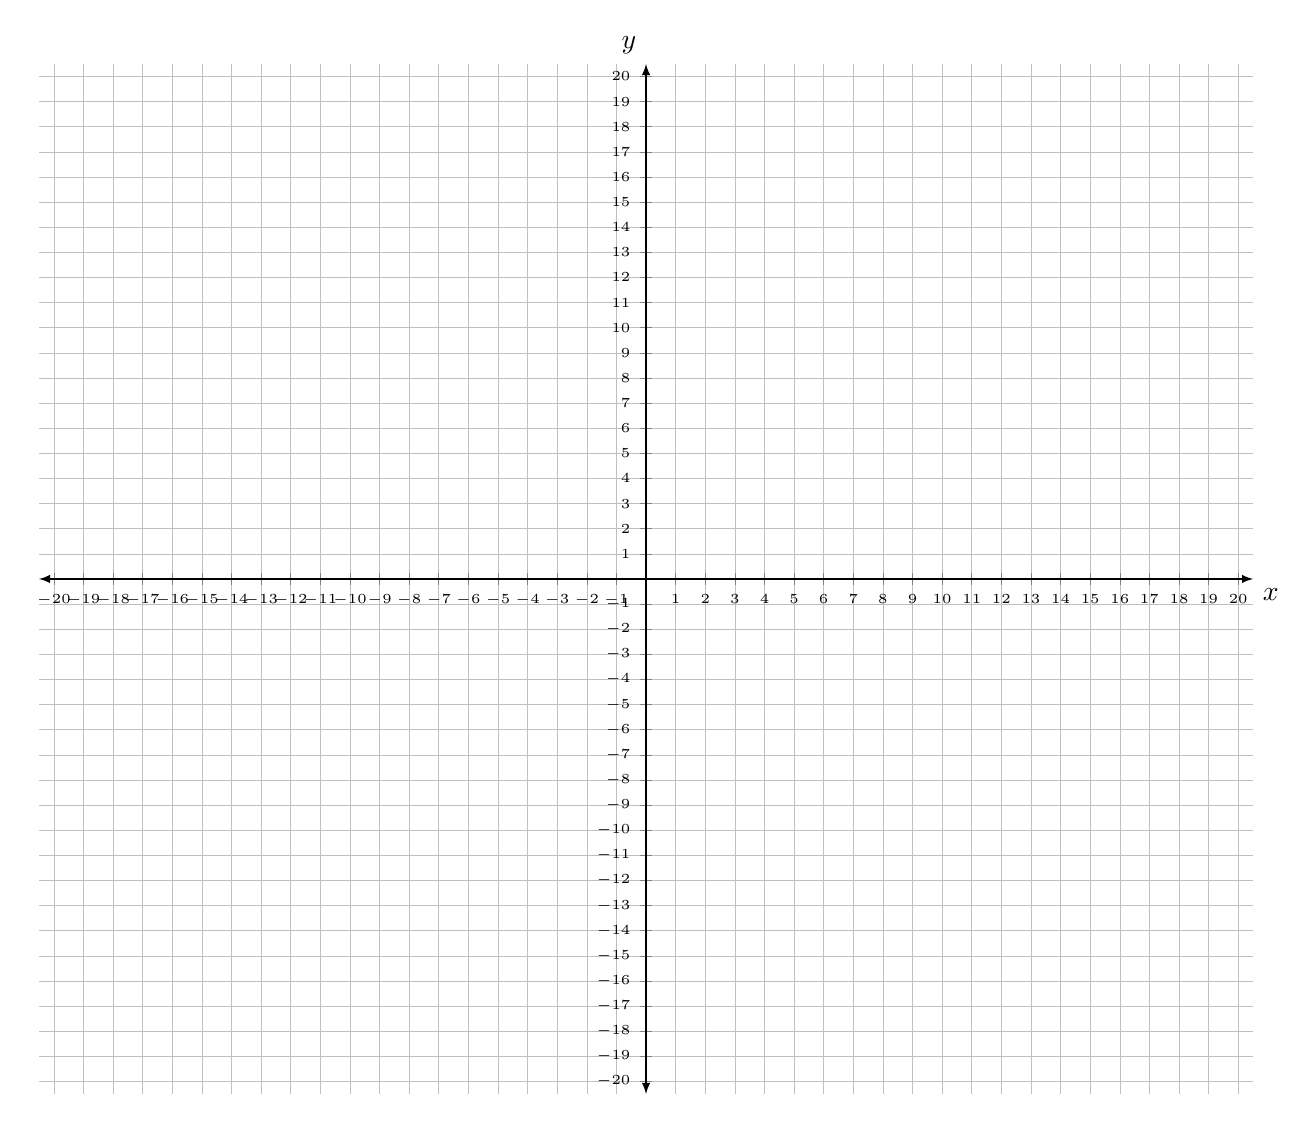
\begin{tikzpicture}[scale=1]
        \begin{axis}[
            axis x line=center,
            axis y line=center,
            xlabel = {$x$},
            ylabel = {$y$},
            xmin=-20,xmax=20,
            ymin=-20,ymax=20,
            xtick distance=1, 
            ytick distance=1, 
            grid=both,
            grid style={line width=.1pt, draw=gray!10},
            major grid style={line width=.2pt,draw=gray!50},
            axis lines=middle,
            axis line style={<->},
            minor tick num=0,
            enlargelimits={abs=0.5},
            axis line style={latex-latex},
            ticklabel style={font=\tiny},
            % ticklabel style={font=\tiny,fill=white},
            % xlabel style={at={(ticklabel* cs:1$(},anchor=north west},
            % ylabel style={at={(ticklabel* cs:1$(},anchor=south west},
            xlabel style={below right},
            ylabel style={above left},
            width=17cm,
        ]
        
        \end{axis}

    \end{tikzpicture}

\end{questions}
 
\end{document}